\documentclass{article}


\usepackage[utf8]{inputenc}
% \usepackage[utf8]{inputenc}
\usepackage{multicol}
\usepackage[a4paper,top=3cm,bottom=3cm,left=2cm,right=2cm,marginparwidth=1.75cm]{geometry}
\usepackage{multicol}
\usepackage{amsmath}
\usepackage{graphicx}
\usepackage{hyperref}
\hypersetup{colorlinks=true,linkcolor=black,filecolor=magenta,urlcolor=cyan,}
\usepackage{amsfonts}
\usepackage{mathtools}
\usepackage{lipsum}
\usepackage{float}


%\renewenvironment{abstract}
% {\quotation\small\noindent\rule{\linewidth}{0.5 pt}\par\smallskip
%  {\centering\bfseries\abstractname\par}\medskip}
% {\par\noindent\rule{\linewidth}{.5pt}\endquotation}





%\title{\textbf{Group Theory-Some basic Definitions and Examples}}
%\author[1]{Anantha Padmanabhan M Nair}
%\affil[1]{\textit{School of Physical Sciences,3rd Year, National %Institute of Science Education and Research, HBNI, Jatni-752050, %India}}


\begin{document}



%Title Page and certificate and acknowlwdgements
\newgeometry{top=5cm,bottom=2.5cm,left=4cm,right=4cm}



\begin{titlepage}

\begin{center}



\textup{\Large {\bf Summer Internship Project} \\ Report}\\[0.3in]

% Title
\Large \textbf {Group Theory}\\[0.7in]


       

% Submitted by
\normalsize Submitted by \\[0.2in]
\textbf{Anantha Padmanabhan M Nair}\\
\normalsize
$3^{rd}$ year Int. MSc Student\\


\includegraphics[width=0.25 \textwidth]{NISER.png}\\[0.1in]
\Large{School of Physical Sciences}\\
\normalsize
\textsc{National Institute of Science Education and Research},\\
Tehsildar Office, Khurda\\
Pipli, Near, Jatni, Odisha 752050\\





\vspace{.2in}
Under the guidance of\\[0.2in]
\textbf{Girish Sharma}\\
Assistant Professor



\vspace{.3in}

% Bottom of the page

\includegraphics[width=0.2\textwidth]{IIT.png}\\[0.1in]
\Large{School of basic Sciences}\\
\normalsize
\textsc{IIT Mandi}\\
Parashar Road, Tehsil Sadar, \\Near Kataula, Kamand, \\Himachal Pradesh, 175005 \\
\vspace{0.2cm}
Summer Internship 2022

\end{center}

\end{titlepage}

\restoregeometry


%Acknowlegdements%Acknowlegdements%Acknowlegdements%Acknowlegdements%Acknowlegdements%Acknowlegdements%Acknowlegdements%Acknowlegdements
\newgeometry{top=6.5cm,bottom=2.5cm,left=6cm,right=6cm}
\cleardoublepage
\begin{center}
    \Large{\textbf{Acknowledgements}}
\end{center}

\vspace{0.2in}
I want to express my profound gratitude to Prof. Girish Sharma, who has served as my mentor and an outstanding role model during this endeavour. I appreciate him allowing me the chance to work with him and guiding me as I discover new ideas and themes. When we talked, he didn't simply explain the subjects; he also taught me how to approach the ideas in a way that wasn't solely based on mathematical proofs. For giving me this chance and inspiring me to investigate, I would also like to thank the School of Basic Sciences at the Indian Institute of Technology, Mandi, and the School of Physical Sciences at the National Institute of Science Education and Research.

\newpage
\restoregeometry
%Acknowlegdements%Acknowlegdements%Acknowlegdements%Acknowlegdements%Acknowlegdements%Acknowlegdements%Acknowlegdements%Acknowlegdements






\newgeometry{top=5cm,bottom=2.5cm,left=4cm,right=4cm}
\newpage
\thispagestyle{empty}

\begin{center}

\huge{School Of Basic Sciences}\\[0.5cm]
\normalsize
\textsc{Indian Institute Of Technology, Mandi}\\[2.0cm]

\emph{\LARGE Certificate}\\[2.5cm]
\end{center}
This is to certify that Mr. Anantha Padmanabhan, Student of National Institute of Science Education and Research, has successfully completed a summer internship in the field of Group Theory from 1/06/2022 to 12/07/2022 under the guidance of Dr.Girish Sharma.We wish him every success in his life and career.\\


IIT Mandi,

Kamand,

Himachal Pradesh
\normalsize 


\vfill


% Bottom of the page
\begin{flushright}
Girish Sharma\\
(Project Guide)\\
\end{flushright}
\begin{flushleft}
Date:
\end{flushleft}

\restoregeometry


%Abstract%Abstract%Abstract%Abstract%Abstract%Abstract%Abstract%Abstract%Abstract%Abstract%Abstract%Abstract%Abstract%Abstract
\newgeometry{top=6.5cm,bottom=2.5cm,left=5cm,right=5cm}

\begin{abstract}
    In this report we will discuss about the basics of the group theory and symmetries.
    The Group Theory is used as a mathematical frame work for describing symmetry properties 
    of classical as well as quantum systems. We will also read about Homomorphisms-a 
    structure-preserving map between two algebraic structures of the same type, 
    Conjugations, and some applications of the Group theory in different fields 
    like the crystallography and Topologies etc. 
    \end{abstract}
\restoregeometry
%Abstract%Abstract%Abstract%Abstract%Abstract%Abstract%Abstract%Abstract%Abstract%Abstract%Abstract%Abstract%Abstract%Abstract


%Content Table Page%Content Table Page%Content Table Page%Content Table Page%Content Table Page%Content Table Page
\pagenumbering{roman}
\newpage
\newgeometry{top=4cm,bottom=2.5cm,left=4cm,right=4cm}
\begin{center}
 \tableofcontents   
\end{center}
\restoregeometry
%Content Table Page%Content Table Page%Content Table Page%Content Table Page%Content Table Page%Content Table Page


%Contents
\newpage

\begin{multicols}{2}
\pagenumbering{arabic}
\section{Introduction}
\subsection{Basic Definition}
In this section we will discuss about the basic definition of the groups. A group is usually denoted by the letter G. its none other than a set along with a defined operator usually called as group multiplication. The group multiplication can be any well defined operation like addition, subtraction etc.The operation is defined as a mapping from G$\times$ G $\longrightarrow$ G.That is this operation must satisfy the below four properties for a set to become a group.This group operation or multiplication is called as group axioms.
\begin{itemize}
    \item Closure Property-Is if a,b $\epsilon$ G and if ab represent the multiplication then ab must also belong to G. 
    \item Associativity- That is the group multiplication must follow
    \begin{equation}
        a(bc)=(ab)c
    \end{equation}
    Where a,b,c$\epsilon$G
    \item Existence of an Identity element-For a group there must be an identity element which satisfies 
    \begin{equation}
       ae=ea=a   
    \end{equation}
    
   for all a $\epsilon$ G
   
   \item Existence of an inverse element- this means that for every element"a" in G there must be an inverse element denoted by $a^{-1}$ which satisfies 
   \begin{equation}
       aa^{-1}=a^{-1}a=e
    \end{equation}
\end{itemize}

\subsection{Examples of groups}
\begin{itemize}
    \item Example:1- Consider the set G which is a set of 4 given 2$\times$2 matrices a,b,c and e and the operation of matrix multiplication. We can see that the set G is a group as it satisfies the above mentioned 4 conditions.
    \begin{center}
    a=
    $\begin{pmatrix}
    0 & -1 \\
    1 & 0 
    \end{pmatrix}$
      b=
     $\begin{pmatrix}
    -1 & 0 \\
    0 & -1 
    \end{pmatrix}$
    c=
    $\begin{pmatrix}
    0 & 1 \\
    -1 & 0 
    \end{pmatrix}$
    
    e=
    $\begin{pmatrix}
    1 & 0 \\
    0 & 1 
    \end{pmatrix}$
    
    Here we can see that
    
    ac=
    $\begin{pmatrix}
    0 & -1 \\
    1 & 0 
    \end{pmatrix}$
    $\begin{pmatrix}
    0 & 1 \\
    -1 & 0 
    \end{pmatrix}$
    =
    $\begin{pmatrix}
    1 & 0 \\
    0 & 1 
    \end{pmatrix}$
    =e
    
    $a^{-1}$=
    $\begin{pmatrix}
    0 & -1 \\
    1 & 0 
    \end{pmatrix}^{-1}$
    =
    c
    =
    $\begin{pmatrix}
    0 & 1 \\
    -1 & 0 
    \end{pmatrix}$
    \end{center}
    \item Example:2- Consider the set of all 2$\times$2 matrices with complex entries with determinant 1. We know that this is an infinite set. Let the operation be ordinary matrix multiplication. Consider the matrix A.
    \begin{center}
      A=
    $\begin{pmatrix}
    a & b \\
    c & d 
    \end{pmatrix}$  
    \end{center}
    
    So the condition is ad-bc=1.We will denote this as SL(2,C). This set is also a group as det(AB)=det(A)det(B) for all the matrices in the set So if A and B belong to the SL(2,C) then AB also belong to the same. We already know that matrix multiplication is Associative. and there is an identity element which is the usual 2x2 identity matrix and inverse of any matrix A is $A^{-1}$ which also belong to SL(2,C).
    \item Example:3- The set O(3) that is the set of all orthogonal transformation in the Euclidean 3-D space which preserve the Euclidean distance. This set is also a group as it satisfies all the properties of the group.
    
\end{itemize}

\subsection{Abelian and Non-Abelian Group}
An Abelian group is one in which the order of application of the group operation does not change the result. in other words for a group G, So for all a,b $\epsilon$ G, then if ab=ba,then the group G is an Abelian group. For example, the set of integers under addition operation is an Abelian group. An the groups which are not Abelian are called Non-Abelian groups. An example would be the rotation group SO(3) in three dimensions (for example, rotating something 90 degrees along one axis and then 90 degrees along a different axis is not the same as doing them in reverse order).





\section{Homomorphism} \label{Homomorphisms}




\subsection{Definition}
So far we have discussed about the definition of groups. Now lets look at Homomorphisms. Consider two groups $G_{1}$ and $G_{2}$. Consider a mapping $\phi$ from $G_{1}$ to $G_{2}$, We say that $\phi$ is a Homomorphism if:
\begin{equation}
    \phi(ab)=\phi(a)\phi(b)
\end{equation}
for all a and b $ \epsilon  G_{1}$

consider an example, consider the Homomorphism from the set $\mathbb{Z}$ to the set $C_{k}$ where the latter is the set of all $k^{th}$ root of unity. The function is given by:
\begin{equation}
    \phi(a)=e^{\frac{2\pi ia}{k}}=\omega^{a}
\end{equation}
We can see that this is a Homomorphism as $\phi(ab)=\phi(a)\phi(b)$ as $\omega^{a+b}=\omega^{a}\omega^{b}$















\subsection{Relation between SL(2,C) and the Lorentz group}
Now we will look at the relation between the SL(2,C) and the Lorentz group. We know that the Lorentz Group is the group of all the 4x4 matrices of Lorentz transformation of the Minkowski space. Minkowski space is the 4-D space (4x1 matrices)including t,x,y and z. Let M denote the 4 dimensional space M=$\mathbb{R}^{4}$. This is set up in such a way that the speed of light is unity. So the magnitude of the 4-D vector is given by:
\begin{equation}
    ||X||^2=x_{0}^{2}-x_{1}^{2}-x_{2}^{2}-x_{3}^{2} 
\end{equation}
 where  
\begin{equation}
X=
\begin{bmatrix}
x_0 \\
x_1 \\
x_2 \\
x_3 
\end{bmatrix}
\end{equation} 
Let L denote the Lorentz group. Consider the Lorentz transformation B which is the linear transformation of M into itself while the Lorentz metric or the magnitude remaining the same, that is $||BX||=||X||$ $\forall$ X $\epsilon$ M. 
Now we will describe a homomorphism from the group SL(2,$\mathbb{C}$). We will map every point in M (X) by a self adjoint 2x2 matrix x which is given by:
\begin{center}

X=
$\begin{pmatrix}
x_0 \\
x_1 \\
x_2 \\
x_3 
\end{pmatrix}$
$\longrightarrow$
$x$=
    $\begin{pmatrix}
    x_0+x_3 & x_1-ix_2 \\
    x_1+ix_2 & x_0-x_3
    \end{pmatrix}$
\end{center}
We can see that, by construction, the x is an Hermitian matrix, that is, its hermitian conjugate is itself. that is $x^{\dagger}=x$. We can also see that the square of the determinant of x is same as that of X ie, 
\begin{equation}
  ||X||^2=det(x)=x_{0}^{2}-x_{1}^{2}-x_{2}^{2}-x_{3}^{2}   
\end{equation}
We know that the matrix $x$ is a self adjoint matrix,  so $x^*=x$. And obviously we can write all of these kind of matrices as a linear combination of the Pauli matrices which are given as:
\begin{center}
    $\sigma_1=$
    $\begin{pmatrix}
    0 & 1 \\
    1 & 0 
    \end{pmatrix}$
    $\sigma_2=$
     $\begin{pmatrix}
    0 & -i \\
    i & 0 
    \end{pmatrix}$
    $\sigma_3=$
    $\begin{pmatrix}
    1 & 0 \\
    0 & -1 
    \end{pmatrix}$
    
    e=
    $\begin{pmatrix}
    1 & 0 \\
    0 & 1 
    \end{pmatrix}$  (The Identity Matrix)
    \end{center}
    
So our defined matrix X can be represented as $x$ which in turn can be represented in terms of Pauli matrices as:
\begin{equation}
    x=x_0e+x_1\sigma_1+x_2\sigma_2+x_3\sigma_3
\end{equation}


Now let us define an actionof the matrix $A$ on the self adjoint matrix $x$ denoted by $\phi (A)x$ and given by:
\begin{equation}
    x \longrightarrow AxA^{*}
\end{equation}
We define the Corresponding Action on the vector $X$ by:
\begin{equation}
    \phi(A)X=AxA
\end{equation}

We can see that since $x$ is a self adjoint matrix, $AxA^*$ is also self-adjoint. Also we can see that the determinants:
\begin{equation}
    det(AxA^{*})=|detA|^{2} \times det(x)
\end{equation}


So, if A is in SL(2,$\mathbb{C}$), then:
\begin{equation}
    ||\phi(A)X||^{2}=||X||^{2}
\end{equation}

and SL(2,$\mathbb{C}$) represents a Lorentz transformation. So we obtain:
\begin{equation}
    \phi(AB)X=\phi(A)\phi(B)X
\end{equation}


So we can prove that $\phi$ is a homomorphism.

Now, let A belong to the subgroup SU(2) of SO(3). So, A is also a unitary matrix. Let $e_0$ be the following matrix:
\begin{center}
    $e_0 =$
    $\begin{pmatrix}
    1  \\
    0  \\
    0  \\
    0  \\
    \end{pmatrix}$
\end{center}  

We can see that:

\begin{equation}
    \phi(A)e_0=e_0
\end{equation}
Since $e_0$ is represented by the identity matrix $I$. Also while restricting the $\phi$ to $SU(2)$, the mapping changes to $SU(2)$ to $O(3)$.

For exapmple. consider the matrix:


\begin{center}
\begin{equation}
U_{\theta}=
{
\begin{pmatrix}
  e^{-i\theta} & 0\\
  0 & e^{i\theta}
\end{pmatrix}
}  
\end{equation}
\end{center}

Now we have:
\begin{center}
\begin{equation}
    \phi({U_{\theta}})X=U_{\theta}xU_{-\theta}=
\end{equation}
\end{center}
\begin{center}
\begin{equation}
=
{
\begin{pmatrix}
  e^{-i\theta} & 0\\
  0 & e^{i\theta}
\end{pmatrix}
} 
{
    \begin{pmatrix}
    x_0+x_3 & x_1-ix_2 \\
    x_1+ix_2 & x_0-x_3
    \end{pmatrix}
}
{
\begin{pmatrix}
    e^{i\theta} & 0\\
  0 & e^{-i\theta}
\end{pmatrix}
}
\end{equation}
\end{center}

We get:
\begin{equation}
 \phi({U_{\theta}})X=
     \begin{pmatrix}
    x_0+x_3 & e^{-i2\theta}(x_1-ix_2) \\
    e^{i2\theta}(x_1+ix_2) & x_0-x_3
    \end{pmatrix}
\end{equation}

We can see that $\phi({U_{\theta}})$ is a rotation about $ x_3 $ axis in the $x_1 - x_2$ plane an Angle of $2\theta$. And as $\theta$ ranges from 0 to $\pi$ the rotation goes from 0 to $2\pi$. 

Similarly, consider the action of the matrix:
\begin{equation}
 V_{\alpha}=
     \begin{pmatrix}
    cos\alpha & -sin\alpha\\
    sin\alpha & cos\alpha
    \end{pmatrix}
\end{equation}

Similarly for the vectors $e_2$ and $e_3$:
\begin{equation}
e_2=
    \begin{pmatrix}
      0\\
      0\\
      1\\
      0\\
    \end{pmatrix}
    \text{and}\;
    e_3=
    \begin{pmatrix}
    0\\
    0\\
    0\\
    1\\
    \end{pmatrix}
\end{equation}

calculating $\phi(V_{\alpha})e_2$ and $\phi(V_{\alpha})e_3$ by the definition of the $\phi$ we get:
\begin{equation}
    \phi(V_{\alpha})e_2=e_2
\end{equation}
So, $\phi(V_{\alpha}$ is the rotation about the $x_2$ axis. and:
\begin{equation}
    \phi(V_{\alpha})e_3=
    {
    \begin{pmatrix}
    cos2\alpha & sin2\alpha\\
    sin2\alpha & -cos2\alpha
    \end{pmatrix}
    }
\end{equation}

This corresponds to the vector:
$
\begin{pmatrix}
0\\
sin2\alpha\\
0\\
cos2\alpha\\
\end{pmatrix}
$
Hence we can see that :
\begin{equation}
   \phi(V_{\alpha})e_3=e_3 cos2\alpha + e_1 sin2\alpha 
\end{equation}
So, we can conclude that the $V_{\alpha}$ is the rotation about the $x_2$ axis by an angle $2\theta$.





\subsection{Representation of Lorentz boost}
Now, Consider the matrix $M_r$ with Real entries Such that $M_r={M_r}^{*}$:
\begin{equation}
    M_{r}=
    {
    \begin{pmatrix}
    r&0\\
    0&\frac{1}{r}
    \end{pmatrix}
    }
\end{equation}

and calculating the $\phi(M_{r})X$ we get:
\begin{equation}
    \phi(M_{r})X=
    \begin{pmatrix}
      r^{2}(x_0 + x_3) & x_1 +ix_2\\
      x_1 -ix_2 & r^{-2}(x_0 - x_3)\\
    \end{pmatrix}
\end{equation}

Here we can see that the $M_r$ doesn't make any change to $x_1 \text{and} x_2$ but the $x_0 \text{and} x_3$ changes as:
\begin{equation}
    x_0' = \frac{r^2 + r^{-2}}{2}x_0 + \frac{r^2 - r^{-2}}{2}x_3
\end{equation}
and
\begin{equation}
    x_3' = \frac{r^2 - r^{-2}}{2}x_0 + \frac{r^2 + r^{-2}}{2}x_3
\end{equation}
Now, the Lorentz boost  in the z direction with parameter t is denoted by $L_t$ and is defined as the transformation:
\begin{equation}
    x_0' = cosh(t)x_0 + sinh(t)x_3
\end{equation}
and
\begin{equation}
    x_3' = sinh(t)x_0 + cosh(t)x_3
\end{equation}
or in matrix form the ${L_t}^z$ is given by:

\begin{equation}
{L_t}^z=
    \begin{pmatrix}
      cosh\;t &0&0&sinh\;t\\
      0&1&0&0\\
      0&0&1&0\\
      sinh\;t &0&0&cosh\;t\\
    \end{pmatrix}
\end{equation}

So, in the preceding section, if we put $r=exp(t)$ in equation 25 and doing the calculation, we can see that :
\begin{equation}
    \phi(M_{e^t})={L_t}^z
\end{equation}
So, till now we have shown that:
\begin{equation}
    \phi(U_{\theta})={R_{\theta}}^z
\end{equation}
\begin{equation}
    \phi(V_{\theta})={R_{\theta}}^y
\end{equation}
\begin{equation}
    \phi(M_{e^t})={L_{2t}}^z
\end{equation}
where ${R_{\theta}}^z \text{and} {R_{\theta}}^y$ are the rotation about z and y axis by an angle $\theta$.





\subsection{Proper Lorentz transformation}


\subsubsection{Definition}
The proper Lorentz transformation is denoted by $L^0$. It is the sub group of $L$ consisting of those transformations which have positive determinant and preserves the foreword light cone, that is, which send each component of the set of time like vectors into itself.


\subsubsection{Lemma}
 The lemma is that, every proper Lorentz transformation,$B$ can be written as:
 \begin{equation}
     B=R_1{L_u}^zR_2
 \end{equation}

Where $R_1$ and $R_2$ are rotations and  ${L_u}^zR_2$ is a lorentz boost in the z-direction.

\subsubsection{Proof:}
By definition we can write:
\begin{equation}
    Be_0=
    {
    \begin{pmatrix}
      x_0\\
      \textbf{x}\\
    \end{pmatrix}
    }
\end{equation}
Where \textbf{x}=$x_1e_1+x_2e_2+x_3e_3$ and $x_0^2-||x||^2=1$. We can find a rotation S in which rotates the vector x to z-axis. So:
\begin{equation}
    SBe_0=
    {
    \begin{pmatrix}
      x_0\\
      0\\
      0\\
      ||x||
    \end{pmatrix}
    }
\end{equation}
the corresponding self-adjoint matrix is:
\begin{center}
$\begin{pmatrix}
  x_0+||\textbf{x}||&0\\
  0&x_0-||\textbf{x}||&0\\
\end{pmatrix}$
\end{center}

Now by choosing r such that:
\begin{equation}
    r^2=\frac{1}{x_0+||\textbf{x}||}
\end{equation}
Then applying $M_r$ gives $\phi(M_r)SBe_0=e_0$. Thus $\phi(M_r)SB=R_2 \;(let)$ is a rotation and we have:
\begin{equation}
    \phi(M_r)SB=R_2
\end{equation}
or we have:
\begin{equation}
    B=S^{-1}[\phi(M_r)]^{-1}] R_1
\end{equation}
With $R_1=S^{-1}$ and $L_{u}^{z}=\phi(M_r)^{-1}$.
So, we have proved the lemma.

\section{Action of a group on a Set}
\subsection{Definition of an Action}
consider a group G and a set M. We will define the \textit{Action} of G on M as a mapping $G\times M \longrightarrow M $. the mapping is defined in such a way that it takes the pair $(a,m)$ to $am$ where $a \epsilon G$ and m and am $\epsilon M$. Which satisfies the associative law:
\begin{equation}
    a(bm)=(ab)m
\end{equation}
and also there there should be an identity element e which gives em=m for any m belonging to M. So, the action of a group on a set M is an homomorphism from the group G to the one-to-one transformation of M. An example could be the action of the group SL(2,$\mathbb{C}$) on the set of Minkowski space which is shown in the above section.

\subsection{Orbit of the point m under action of G}
The orbit of the point m is denoted by $G\cdot m$, this set is defined as:
\begin{equation}
    G\cdot m=\{x|x\epsilon M \; \text{such that} \; x =am \; \forall \; a\epsilon G , \; m\epsilon M \; \}
\end{equation}
That is, let G act on M ans let $m$ be a point in M, then the orbit of $m$ is defined as the subset of M in which the elements are of the form of all am for all a belonging to G and m belonging to M.

For example, Consider the action of the group SO(3) on the set of all points in the 3-Dimensional Euclidean space. We know SO(3) is the group of all the rotations in the space which conserves the length or the magnitude of the vector to that point. So by definition of the orbit, orbit of any point in the space except the origin is the collection of all points equidistant from the origin, that is its a sphere centered at the origin and the orbit of the origin is only the origin itself because the result of rotation of origin is the origin itself.


\subsection{Isotropy Group of point m}
The orbit group of point $m$ is a sub set of the $G$ denoted by $G_m$ which is defined as:
\begin{equation}
    G_m = \{ x | \; xm=m \; \forall \; m  \epsilon M\; \text{and} \; x\; \epsilon G \;\}
\end{equation}
Here, $G$ acts on $M$, and the isotropy group of $m$ is the set of all points in $G$ that preserves the point $m$. For example, the group SO(3) acts on the 3-D space. consider a point $ m\neq 0$. So the isotropy group of the point m is the set of all rotations which is about the point m. So, the $m$ is preserved. The isotropy group of the point $m=0$ that is the origin is the whole group of SO(3).

Let $\#G$ denote the number of elements in the group $G$. let $G$ act on $M$, consider a point $m$ in M, consider the orbit of $m$ under G. the number of elements in the orbit group of m is given by $ \# ( G\cdot m ) $. So, if $n$ is an element in $G\cdot m$, then $n=am$ for some a in G. If n=bm as well then $a^{-1}b$ must lie in $G_m$. So, this means that to every element n there are $\#G_m$ elements which map m to n.
So we can write:
\begin{equation}
    \#G = \# G \cdot m \times \# G_m
\end{equation}

\subsection{Cosets}

We say that G acts transitively on M if M has only a single orbit. The coset is denoted by $aG_{m}$  defined as:
\begin{equation}
   aG_m= \{ab \; | \; \forall \;b\; in\; G_m\}    
\end{equation}
Each coset contains the same number of elements as the subgroup $G_m$. The subgroup $Gm$'s number of elements is shared by all cosets. The point am may be identified with the coset $aG_m$, which is made up of all group elements that transport the point m into the point am. Since G operates transitively on M, there exists at least one element b of G such that n=bm for each element n of M. As a result, we have connected every point of M with a coset of G. We may identify the set of cosets by using the notation $G/G_m$ ~\cite{sternberg1995group}



\section{Conjugation and Conjugacy Classes}
We saw the action of G on a set m. Now lets consider the action of G on itself. When G acts on itself by left multiplication, a  transforms b into ab, this transformation is always transitive.


The action of G on itself is called a conjugation if the action takes "b" to $aba^{-1}$. Conjugation always defines a group action, since the action of ac on b yeilds . 
\begin{equation}
    (ac)b(ac)^{-1}=a(cbC^{-1})a^{-1}
\end{equation}
which is same as the action of c followed by action of a on b.
 Now the orbits of these groups under conjugation are called \textit{Conjugacy classes} of the group. The condition for 2 elements to belong to the same group is that, there exist some a such that:
 \begin{equation}
     aba^{-1}=c
 \end{equation}
from this, we can make 2 conclusions:
\begin{enumerate}
    \item The identity is always a one element conjugacy class as $aea^{-1}=a$ for any a.
    \item For an Abelian group, every element is in a conjugation class by itself as $aba^{-1}=aa^{-1}b=b$ since G is an Abelian group.
\end{enumerate}

\section{Applications to crystallography}
The notion of form in crystallography can be clarified using the concept of orbits. The ordinary salt forms cubic crystals if it is allowed to crystallize under controlled suitable conditions. We can consider the cube as its in $\mathbb{R}^3$ denoted by C, with its vertices at $(\pm1, \pm1,\pm1)$. Let the group of all orthogonal transformation which carry C into itself be denoted by $O_{h}$. The only linear transformations that preserve the cube are the ones that takes the $(x,y,z)$ to $(u,v,w)$ where u,v,w are the permutations of $\pm x,\pm y, \pm z$. Now $\pm$ can be distributed to x,y or z. So there are $2^3$ choices of $\pm$ and there are $3!$ ways of permuting the x.y and z. So, the total number of elements in $O_{h}$ is $2^3 \times 3!=48 $.

Now if we add urea to the NaCl crystals, then at the corners of the cube, small equilateral congruent triangle starts to form. Since the triangles are congruent, the crystal is still invariant under $O_h$. As the amount of urea increases, the size of the triangles increases and the faces become hexagons, and finally it becomes an octahedron. The group preserving the octahedron is same as the one preserving the cube hence the name $O_{h}$. 

In order to get the cubic crystals, one has to make it in carefully controlled conditions. Normally formed crystals are irregular in shape but in some sense it exhibits symmetry. The transition of the cube as the amount of urea increases in shown in figure 1 a$\longrightarrow$d. But the angles between the corresponding sides of all the crystals Will be same as its given by Nicolas steno and Christian Huygens as the "Law of corresponding angles".

\begin{figure}[H]
    \centering
    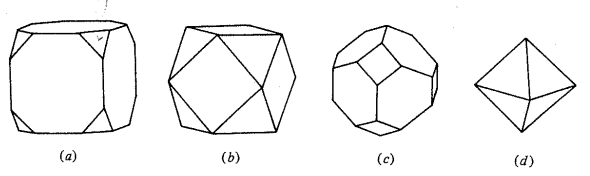
\includegraphics[width = 7.5cm]{fig1.png}
    \caption{Action of urea on the NaCl crystal~\cite{sternberg1995group}}
    \label{fig1}
\end{figure}

We can better understand what crystallographers mean when they talk about a crystal's "shape" by using the concept of an orbit of a group action. The observable symmetry of a crystal is best described in terms of directions, as we have already stated. The collection of normal directions to the faces, according to the law of the constancy of matching angles, is what is invariant (up to an overall rotation). Even though the crystal may have a somewhat uneven exterior, these instructions apply to all crystals of the same composition. These directions can be thought of as points on the unit sphere. This collection of points is affected by the crystal's group of symmetries. \textit{An orbit of the symmetry group acting on this set of directions is what is called a form of the crystal}
\section{The Topology of \textit{SU(2)} and \textit{SO(3)}}

Now in this section, we will discuss about the structure of the group SO(3). Let m $\epsilon$ $M$ and $a \; \epsilon \;G$. A group element c lies in $G_{am}$ if and only if:
\begin{equation}
  c=aba^{-1}  \;\text{where}\; b \; \epsilon \; G_{m}
\end{equation}
mathematically:
\begin{equation}
    G_{am}=aG_{m}a^{-1}
\end{equation}
Then if $b$ is in $G_{m}$ (So that, $bm=m$, then $c(am)=(aba^{-1)}am=abm=am$ so that $c$ is in $G_{am}$. Now using this, its converse and the concept of Euler's angle, we will prove the mapping $\phi$ in section of Section-2 \ref{Homomorphisms} where we took SU(2) to all of SO(3). In the Euler's description, any arbitrary element of \textit{SO(3)} can be written a product of 3 rotations:
\begin{equation}
    R={R^{z}}_{\phi}{R^{y}}_{\theta}{R^{z}}_{\psi}
\end{equation}
Where the axis of rotation is denoted by the superscript and the angle by which the rotation is made is denoted by the subscript. Here $\psi,\;\theta,\; \text{and}\; \phi$ are called the \textit{Euler angles}. Once we got this kind of composition, we can now construct a matrix in $SU(2)$ which maps into product of any such rotation. Now, lets prove the Euler's theorem. Lets consider a unit sphere and let its north pole be $n$. The rotation R is completely determined by a the knowledge of the image $Rn$ of n and of the image of any unit tangent vector to the sphere passing through $n$~\cite{sternberg1995group}. 
If B is in the isotropy group of $SO(3)_R{n}$, then C is some rotation which satisfy $R=CB$ with, $CBn=Bn$ where B is some other rotation which satisfy $Rn=Bn$.  So we can get n to any other point on the unit sphere (namely $p=Rn$) by first applying rotation about the y-axis and then rotating about the z-axis. considering $p=Rn$, we van write:
\begin{equation}
    Rn={R^{z}}_{\phi}{R^{y}}_{\theta}n
\end{equation}
That is, $Rn=Bn$ with $B={R^{z}}_{\phi}{R^{y}}_{\theta}$. But this means $R=CB$, where C is in $SO(3)$
, so $C=BDB^{-1}$, Where $D$ is in $SO(3)_R{n}$. Thus D is a rotation about the z-axis, i.e. $D={R^{z}}_{\psi}$ for some $\psi$ ~\cite{sternberg1995group}. So we have:
\begin{equation}
  R=BDB^{-1}B=BD={R^{z}}_{\phi}{R^{y}}_{\theta}{R^{z}}_{\psi}  
\end{equation}
Hence the Euler's theorem is proved.

Now using these we will study some topological properties of the group SO(3). We know that every element of the $SU(2)$ can be written in the form of the matrix 
$\begin{pmatrix}
a&b\\
-b^{*}&a^{*}\\
\end{pmatrix}$
where $|a|^{2}+|b|^{2}=1$. Now writing $a=y_1-iy_2$ and $b=y_3-iy_4$, then the $y_i$'s represent a unit sphere in the 4-D y space with:
\begin{equation}
    y_{1}^{2}+y_{2}^{2}+y_{3}^{2}+y_{4}^{2}=1
\end{equation}
Here the Identity element e corresponds to $(1,0,0,0)$.

Now the sphere in any positive dimension has the property that it can shrink any closed curve to a single point. So, lets consoder a curve $\gamma(t)$ with $ \gamma (1) =\gamma (0) = e $.We can move the curve a little bit so that $\gamma$ does not pass through the point $(-1,0,0,0)$ for any $t$. NOw, we can continuously deform the curve by a constant map by pushing each point in the curve along the great circle fron south polw i.e. $(-1,0,0,0)$ to the north pole $(1,0,0,0)$. Now we say that $SU(2)$ is \textit{simply connected}. 

Now for the group $SO(3)$, consider a rotation through an angnle t about the z-axis. This Rotation $R_{t}^{z}$ describes a closed curve in $SO(3)$ as t ranges from $0$ to $\pi$. Now we will prove that this curve cannot be decomposed to a curve in $SO(3)$. We can consider the pre-image of this curve in $SU(2)$, and let it be $C(t)$ with $C(0)=e$ and also C is continuous and $\phi(C(t))=R_{t}^{z}$. We know that $\phi$ is two-to-one and that the two points that maps to the same point in $SO(3)$ are antipodal points on the 3-D sphere. As C its continuous, C gets fixed completely and it is the semi circle in the $y_3=y_4=0$ plane given by $y_1(t)=\cos(t/2)$ ans $y_2(t)=\sin(t/2)$. Thus, $C(2\pi)=-e$. By, using continuity, we can see that this is in fact true for any curve. That is for any curve $B(s,t)$ in $SO(3)$ with $B(s,0)=B(s,2\pi)=\;identity\;element\;$ and if $B(0,t)=R_{t}^{z}$, then we can find a curve $C(s,t)$ in $SU(2)$ such that C depends continuously on s and t and has the values in SU(2) with $\phi(C(s,t)=B(s,t)$. Then by the arguments same as abive we can show that $C(s,2\pi)=-e$. IN this way we can see that there is no way of shrinking the curve $R_{t}^{z}$ to the constant curve, i.e. there cannot be any continuous B with B(1,t) identically equal to the identity element in SO(3).

So, we have shown that the curve consisting of a family of rotations about an axis traversed once from 0 to$\pi$ cannot be deformed to a point while the same curve when traversed twice can be shrunk to a point.
\section{Conclusion}

So far in this report we 1st discussed and learned about the basic definition of the Groups and saw some examples, then we discussed about the mappings from and to the groups, Homomorphisms, Action, conjugation etc and in the last part we saw some application of the group theory in some Fields like the Crystallography and in the topology of some groups namely SO(3). We were able to study and prove some of the basic theorems and formulas in the group theory like in the Lorentz transformations, Lorentz Boosts, etc. So, Finally, we could see that the group theory has many applications in physics and Chemistry.
\end{multicols}




\bibliographystyle{plain}
\bibliography{bib.bib}


\end{document}